\documentclass[12pt]{article}
\usepackage{amsmath}
\usepackage{booktabs}
\usepackage{graphicx}

\title{Discrete Assignment-11.9.1-11}
\author{Hiba Muhammed \\
        EE23BTECH11026}
\date{} 
\begin{document}

\maketitle

\section*{Problem Statement}
Write the first five terms in the sequence:
\begin{align}
a_{0}  &= 3 \\
a_{n}  &= 3a_{n-1} + 2 \quad \text{for } n > 0
\end{align}

\section*{Solution}
\begin{table}[h]
  \centering
  \caption{Input Parameters: First Term and General Formula}
  \begin{tabular}{|c|c|}
    \hline
    \textbf{Term} & \textbf{Value} \\
    \hline
    \(x(0)\) & 3 \\
    \(x(n)\) & \(3x(n-1) + 2\) \\
    \hline
  \end{tabular}
\end{table}


So, the first 5 terms of the sequence are \(3, 11, 35, 107, 323\).

\subsection*{Difference Equation and Z-transform}

\begin{align}
x(n) - 3x(n-1) &= 2 \\
\text{ Z-transform of equation :} \nonumber \\
X(z) &= \frac{2}{(1 - z^{-1})(1 - 3z^{-1})} \\
&= \frac{A_1}{1 - z^{-1}} + \frac{A_2}{1 - 3z^{-1}}
\end{align}

\begin{align}
2 &= A_1(1-3z^{-1}) + A_2(1-z^{-1})
\end{align}

\begin{align}
A_1 &= -1 \\
A_2 &= 3
\end{align}

Substitute these values back into the modified partial fraction decomposition:
\begin{align*}
X(z) &= -\frac{1}{1-z^{-1}} + \frac{3}{1-3z^{-1}}
\end{align*}


\begin{figure}[h]
    \centering
    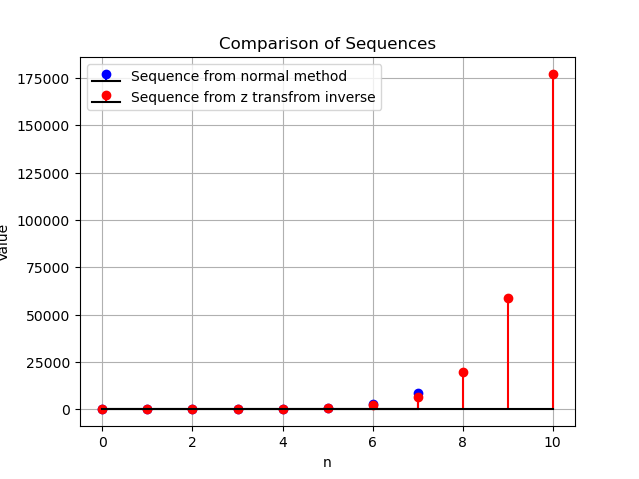
\includegraphics[width=0.8\textwidth]{Figure_1.png}
    \caption{Comparison of Sequences}
    \label{fig:comparison}
\end{figure}

\end{document}

